\section{Computational Complexities of the Algorithms}

\lettrine[nindent=0em,lines=3]{I}n this chapter we will briefly discuss each one of the algorithms intended to be used in the development of the Intelligent HVAC System. Along with the description of such algorithms we will present a very brief analysis on their computational complexity.

\subsection{Artificial Neural Network}

Artificial Neural Networks (ANNs) are computing systems inspired by the biological networks that constitute the brain. Such systems learn (progressively improve performance) to do tasks by considering examples, generally without task-specific programming. 

An ANN is based on a collection of connected units called artificial neurons, (analogous to axons in a biological brain). Each connection (synapse) between neurons can transmit a signal to another neuron. The receiving (postsynaptic) neuron can process the signal(s) and then signal downstream neurons connected to it. Neurons may have state, generally represented by real numbers, typically between 0 and 1. Neurons and synapses may also have a weight that varies as learning proceeds, which can increase or decrease the strength of the signal that it sends downstream. Further, they may have a threshold such that only if the aggregate signal is below (or above) that level is the downstream signal sent. Typically, neurons are organized in layers. Different layers may perform different kinds of transformations on their inputs. Signals travel from the first (input), to the last (output) layer, possibly after traversing the layers multiple times. \cite{ann_wikipedia}

The multilayer perceptron is an artificial neural network structure and is a nonparametric estimator that can be used for classification and regression. It is a supervised learning algorithm that learns a function $f(\cdot): R^m \rightarrow R^o$ by training on a dataset, where $m$ is the number of dimensions for input and $o$ is the number of dimensions for output. Given a set of features $X = {x_1, x_2, ..., x_m}$ and a target $y$, it can learn a non-linear function approximator for either classification or regression. It is different from logistic regression, in that between the input and the output layer, there can be one or more non-linear layers, called hidden layers. Figure \ref{Fig:mlp_example} shows a one hidden layer MLP with scalar output. \cite{ann_scikit}

\begin{figure}[H]
\centering 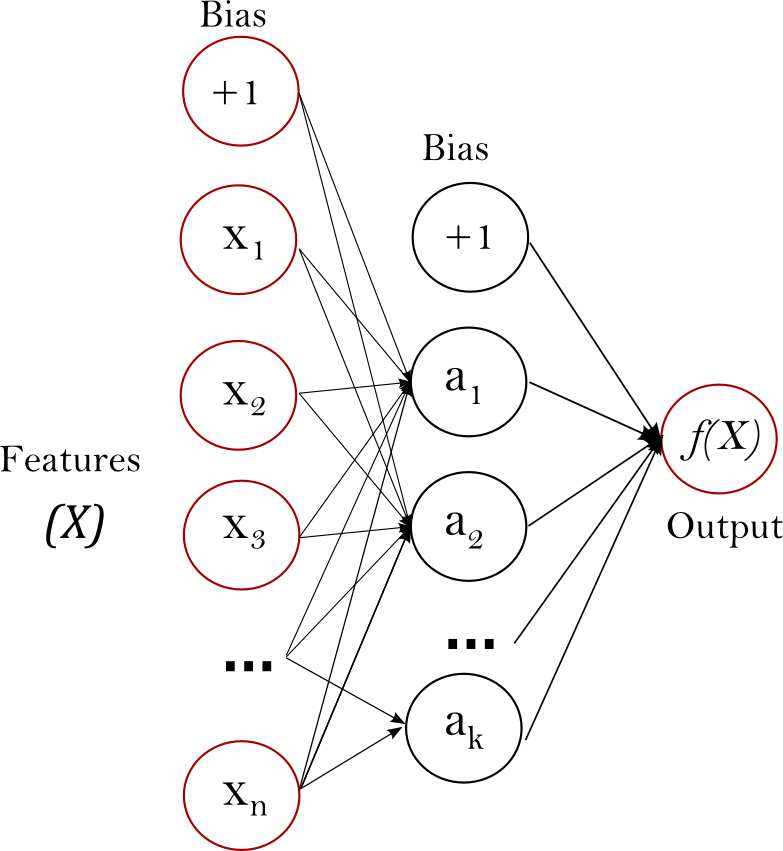
\includegraphics[width = 60mm, height = 60mm]{imgs/multilayerperceptron_network.png}
\caption{Multilayer perceptron}
\label{Fig:mlp_example}
\end{figure}

The leftmost layer, known as the input layer, consists of a set of neurons $\{x_i | x_1, x_2, ..., x_m\}$ representing the input features. Each neuron in the hidden layer transforms the values from the previous layer with a weighted linear summation $w_1x_1 + w_2x_2 + ... + w_mx_m$, followed by a non-linear activation function $g(\cdot):R \rightarrow R$ - like the hyperbolic tan function. The output layer receives the values from the last hidden layer and transforms them into output values.

The advantages of multilayer perceptrons are:
 \begin{itemize}
 \item Capability to learn non-linear models
 \item Capability to learn models in real-time (on-line learning)
 \end{itemize}
 
 The disadvantages of multilayer perceptron (MLP) include:
 \begin{itemize}
 \item MLP with hidden layers have non-convex cost function where there exists more than one local minimum. Therefore different random weight initializations can lead to different validation accuracy.
 \item MLP requires the tuning number of of hyperparameters such as the \textit{number of hidden neurons, layers and iterations}.
 \item MLP is sensitive to feature scaling
 \end{itemize}
 
 \subsubsection{Computational Complexity}
 
Suppose there are $n$ training samples, $m$ features, $k$ hidden layers, each containing $h$ neurons - for simplicity, and $o$ output neurons. The time complexity of the feedforward-backpropagation algorithm is 

\begin{equation}
O(n\cdot m \cdot h^k \cdot o)
\label{eq:ann_complexity1}
\end{equation}

Also for the sake of simplicity lets assume that $m>h>o$, hence the time complexity for feedforward-backpropgation algorithm is 

\begin{equation}
O(n\cdot m^{k+2})
\label{eq:ann_complexity2}
\end{equation}

Additional to the computation of the gradients using the backpropagation algorithm we need to consider the complexity (convergence ratio) of the algorithm used for solving the minimization problem inherent to the neural network, recall that at each iteration a minimization problem is solved. For the best case, this is superlinear (L-BFGS) and for the worst case it is linear (Stochastic Gradient Descent).

\subsection{Anomaly Detection}
\label{sec:anomaly_detection_alg}

Assume we have a sample $\mathbb{M}$ drawn from the same distribution. An outlier, novelty, or anomaly is an instance that is very much different from other instances in the sample. An outlier may indicate an abnormal behavior of the system; for example, in a dataset of credit card transactions, it may indicate fraud; in an image, outliers may indicate anomalies, for example, tumors. \cite{intro_to_machine_learning}

Outlier detection is not generally cast as a supervised, two-class clas- sification problem of seperating typical instances and outliers, because generally there are very few instances that can be labeled as outliers and they do not fit a consistent pattern that can be easily captured by a two- class classifier. Instead, it is the typical instances that are modeled; this is sometimes called one-class classification. Once we model the typical instances, any instance that does not fit the model (and this may occur in many different ways) is an anomaly.

Outlier detection basically implies spotting what does not normally happen; that is, it is density estimation followed by checking for in- stances with too small probability under the estimated density. As usual, the fitted model can be parametric, semiparametric, or nonparametric. In the parametric case, for example, we can fit a Gaussian to the whole data and any instance having a low probability, or equally, with high Mahalanobis distance to the mean, is a candidate for being an outlier. \cite{anomaly_scikit}

Figure \ref{Fig:noveltyDetection_example} shows how novelty detection can separate data into regular observations and abnormal observations.

\begin{figure}[H]
\centering 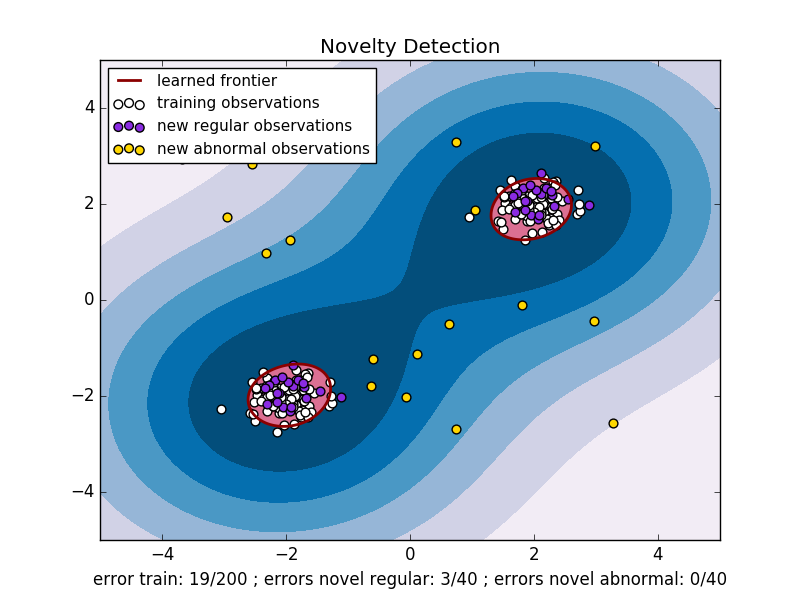
\includegraphics[width = 90mm, height = 40mm]{imgs/noveltyDetection.png}
\caption{Novelty detection}
\label{Fig:noveltyDetection_example}
\end{figure}

One common way of performing outlier detection is to assume that the regular data come from a known distribution (e.g. data are Gaussian distributed). From this assumption, we generally try to define the “shape” of the data, and can define outlying observations as observations which stand far enough from the fit shape. The process for defining the "shape" of the data is as follows and assumes that all of the samples come from a known distribution, say Gaussian for the purposes of this explanation.

Assume a training set $T = \{x^{(1)}, \cdots, x^(m) \}$ where $x \in \mathbb{R}^n$. Suppose that each feature $x_i from x$ is distributed according to some Gaussian distribution $x_i \sim \mathcal{N}(\mu_i, \sigma_i^2)$. Hence $p(x) = \prod_{j = 1}^n p(x_j; \mu_j, \sigma_j^2)$. The task is now to find the corresponding means $\mu_i$ for $i = 1,\cdots,n$ and standard deviations $\sigma_i^2$ for  $i = 1,\cdots,n$ of the $n$ different distributions. This can be easily done for the Gaussian distribution as follows

\begin{equation}
\mu_j = \frac{1}{m} \sum_{i=1}^{m} x_j^{(i)}
\label{eq:mean_eq_gaussian}
\end{equation}

and

\begin{equation}
\sigma_j^2 = \frac{1}{m} \sum_{i=1}^{m} (x_j^{(i)} - \mu_j)^2
\label{eq:std_eq_gaussian}
\end{equation}

We can now describe the simplest anomaly detection algorithm

\begin{enumerate}
\item Choose features $x_i$ that might be indicative/sensitive of/to anomalies.
\item Fit parameters $\mu_1, \cdots, \mu_n$ and $\sigma_1^2,\cdots, \sigma_n^2$ using equations \eqref{eq:mean_eq_gaussian} and \eqref{eq:std_eq_gaussian} respectively.
\item Given a new example $x$, compute $p(x) = \prod_{j = 1}^n p(x_j; \mu_j, \sigma_j^2)$ 
\item Tag the new sample $x$ as an anomaly if $p(x) < \epsilon$, where $epsilon$ is a hyperparameter defined by the user.
\end{enumerate}

 \subsubsection{Computational Complexity}

Usually the complexity of this algorithm is negligible compared to the complexity of the feedforward-backpropagation algorithm. As can be seen from the Algorithm in Section \ref{sec:anomaly_detection_alg} the asymptotic complexity of such algorithm is $O(n)$ where $n$ is the number of choosen features.